%\begin{figure*}[t]
%		\begin{minipage}{0.32\linewidth}
%			\centering
%			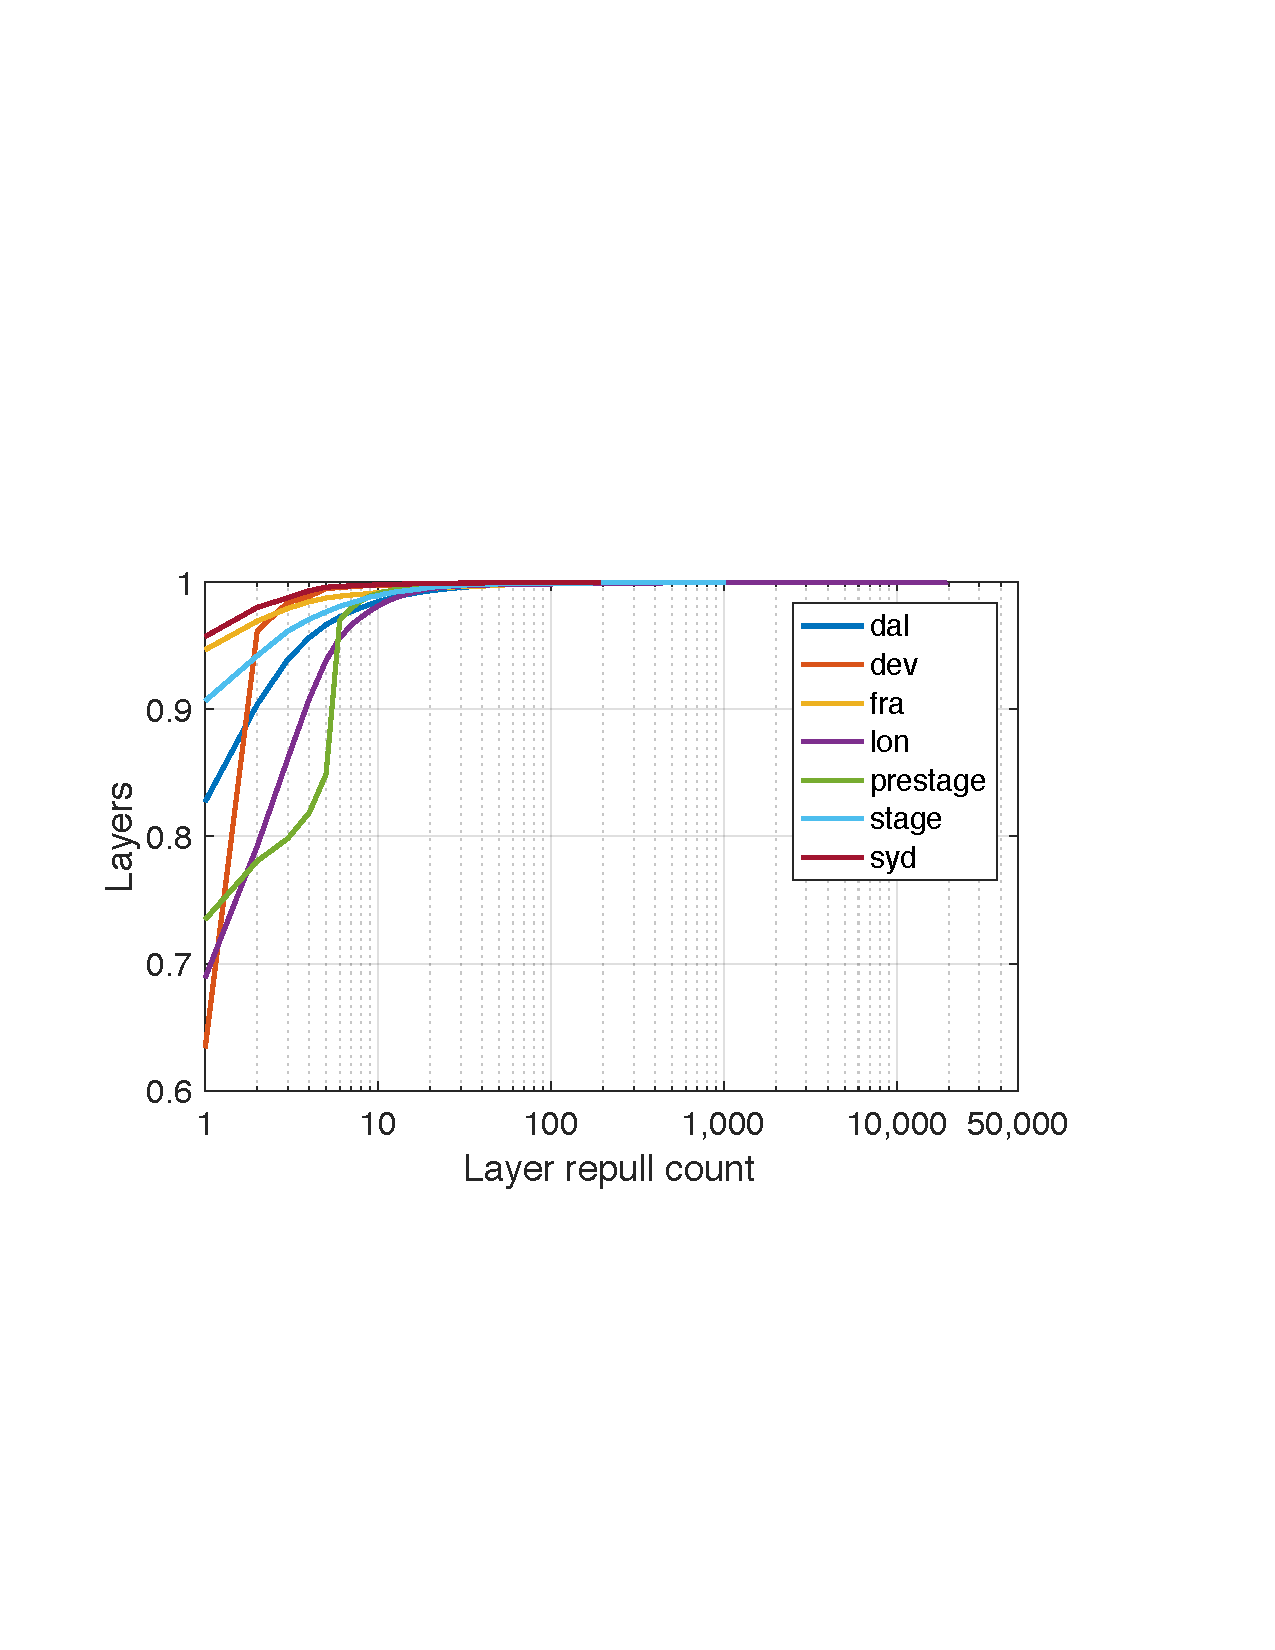
\includegraphics[width=1\textwidth]{graphs/cdf-layer-repull-by-same-client.pdf}
%			%\caption{CDF of layer repull count.}
%		%	\vspace{-3pt}
%			\label{fig:layer-repull-cdf}
%		\end{minipage}
%			\begin{minipage}{0.32\linewidth}
%				\centering
%				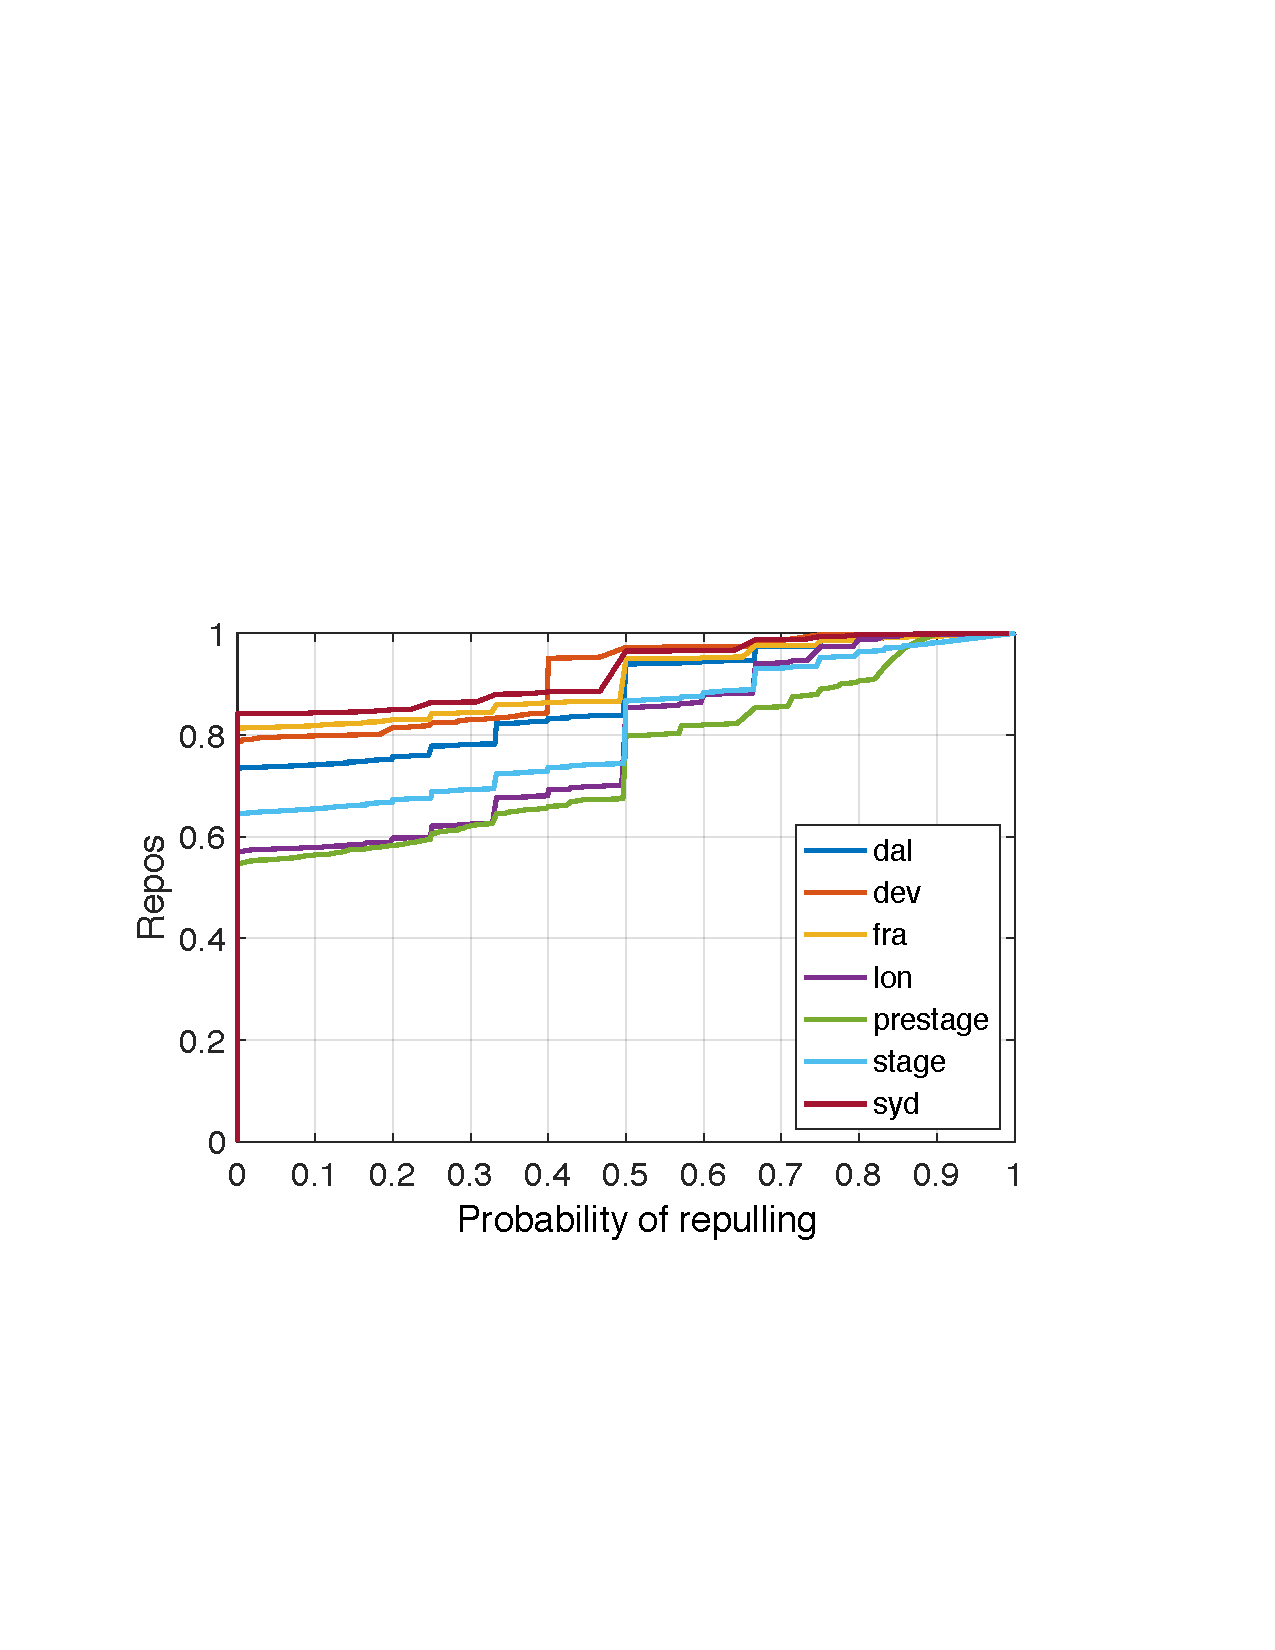
\includegraphics[width=1\textwidth]{graphs/cdf-repo-repull-ratio-by-same-client.pdf}
%				%\caption{PDF of repository repulling probability.}
%				%	\vspace{-3pt}
%				\label{fig:repo-repull-cdf}
%			\end{minipage}
%		\begin{minipage}{0.32\linewidth}
%			\centering
%			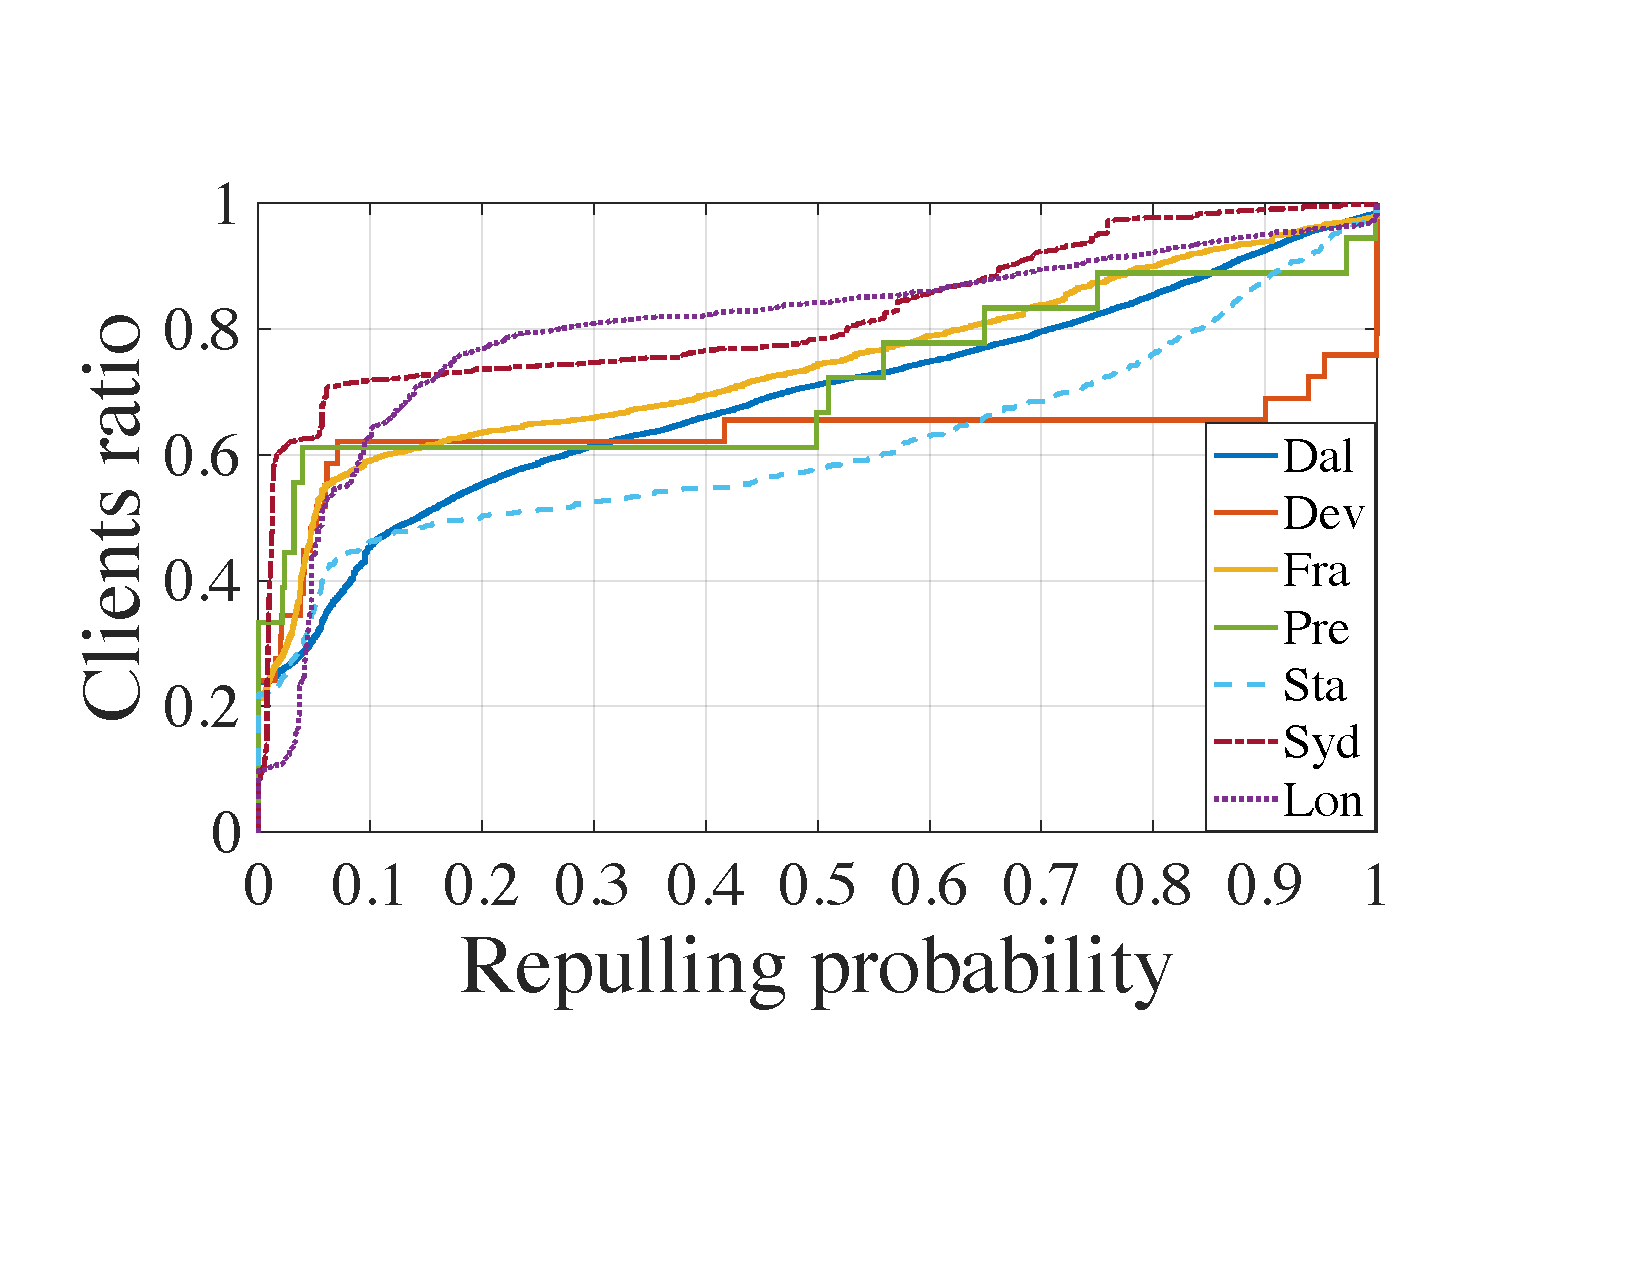
\includegraphics[width=1\textwidth]{graphs/cdf-client-repull-layer-request-ratio.pdf}
%			%
%			%	\vspace{-3pt}
%			\label{fig:client-repull-cdf}
%		\end{minipage}
%	\caption{PDF of client repull count, repository repulling probability, and client repulling probability..}
%\end{figure*}

%\begin{figure}[!t]
%	\centering
%	\subfigure[\texttt{GET} layer request count]{
%		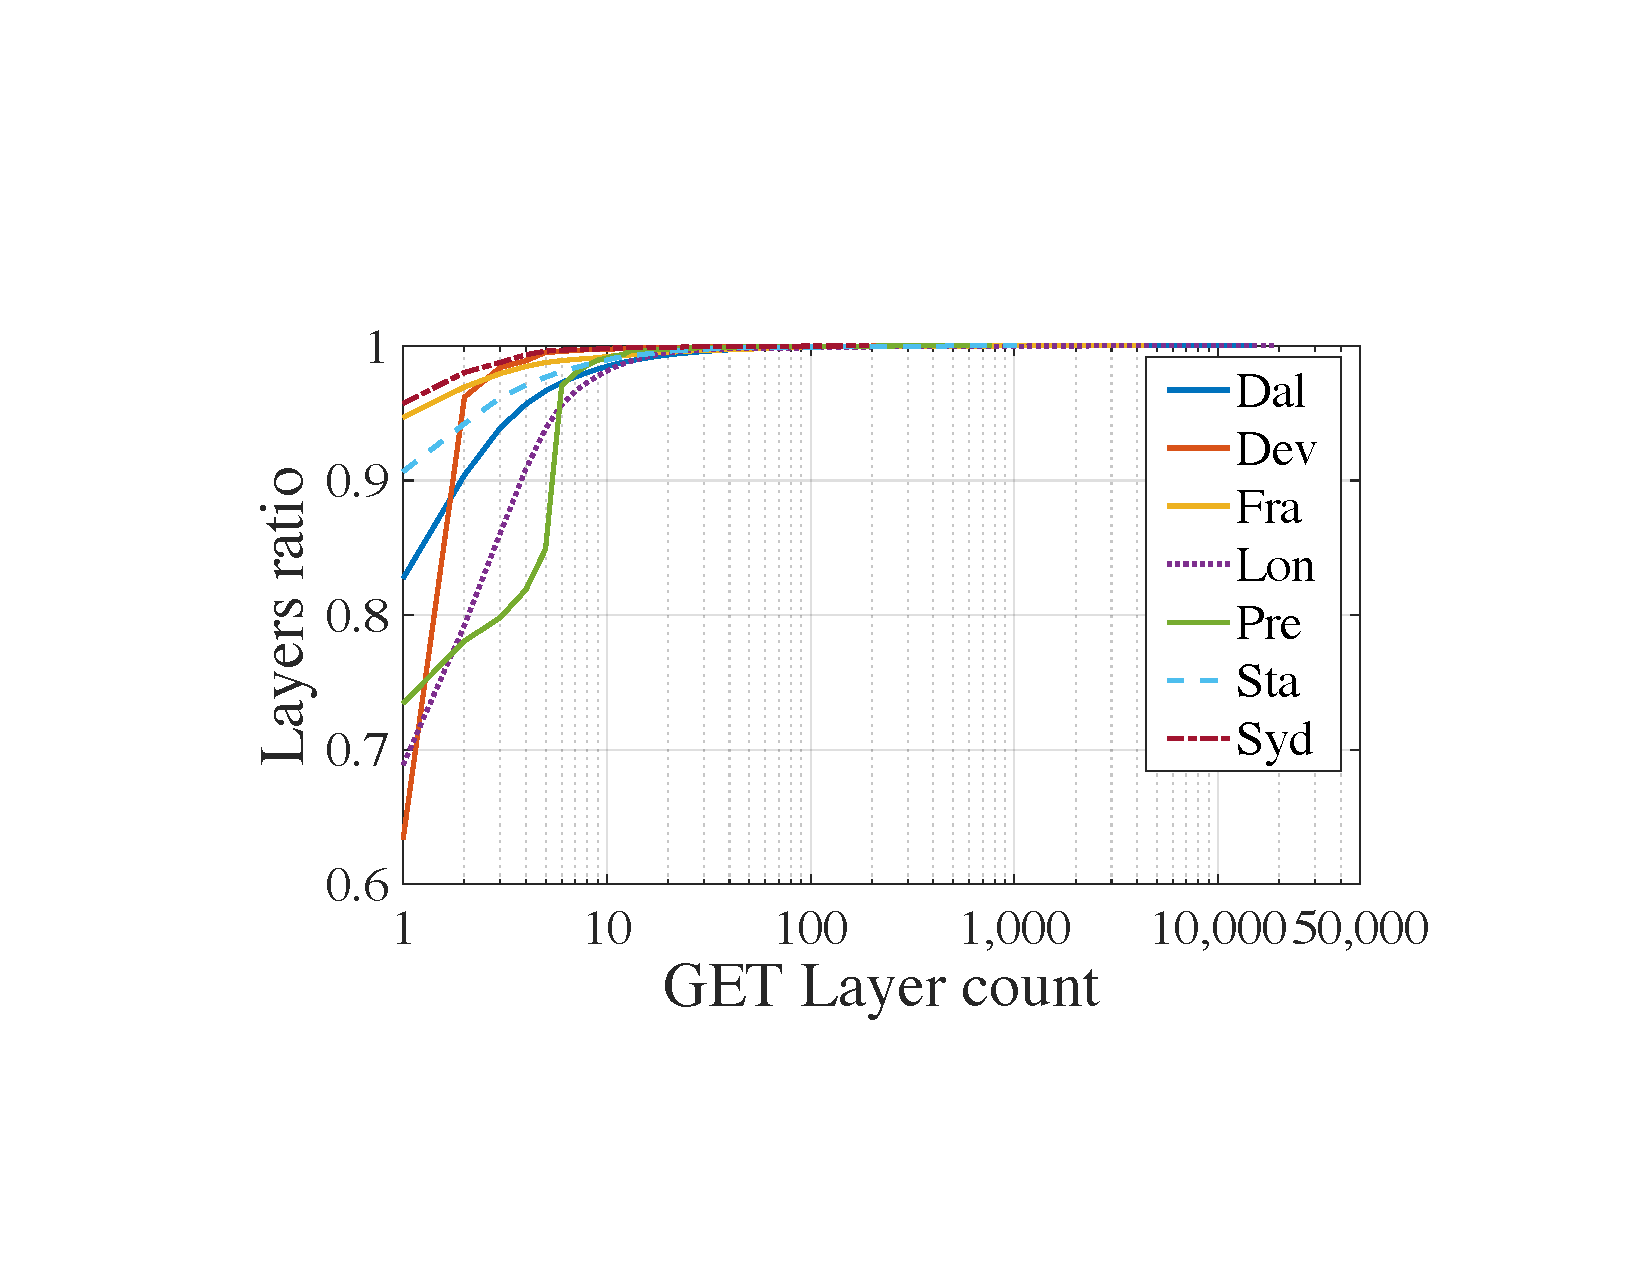
\includegraphics[width=0.22\textwidth]{graphs/cdf-layer-repull-ratio-by-same-client.pdf}
%		\label{fig:layer-repull-cdf}
%	}
%%	\subfigure[Repository repulling probability]{
%%		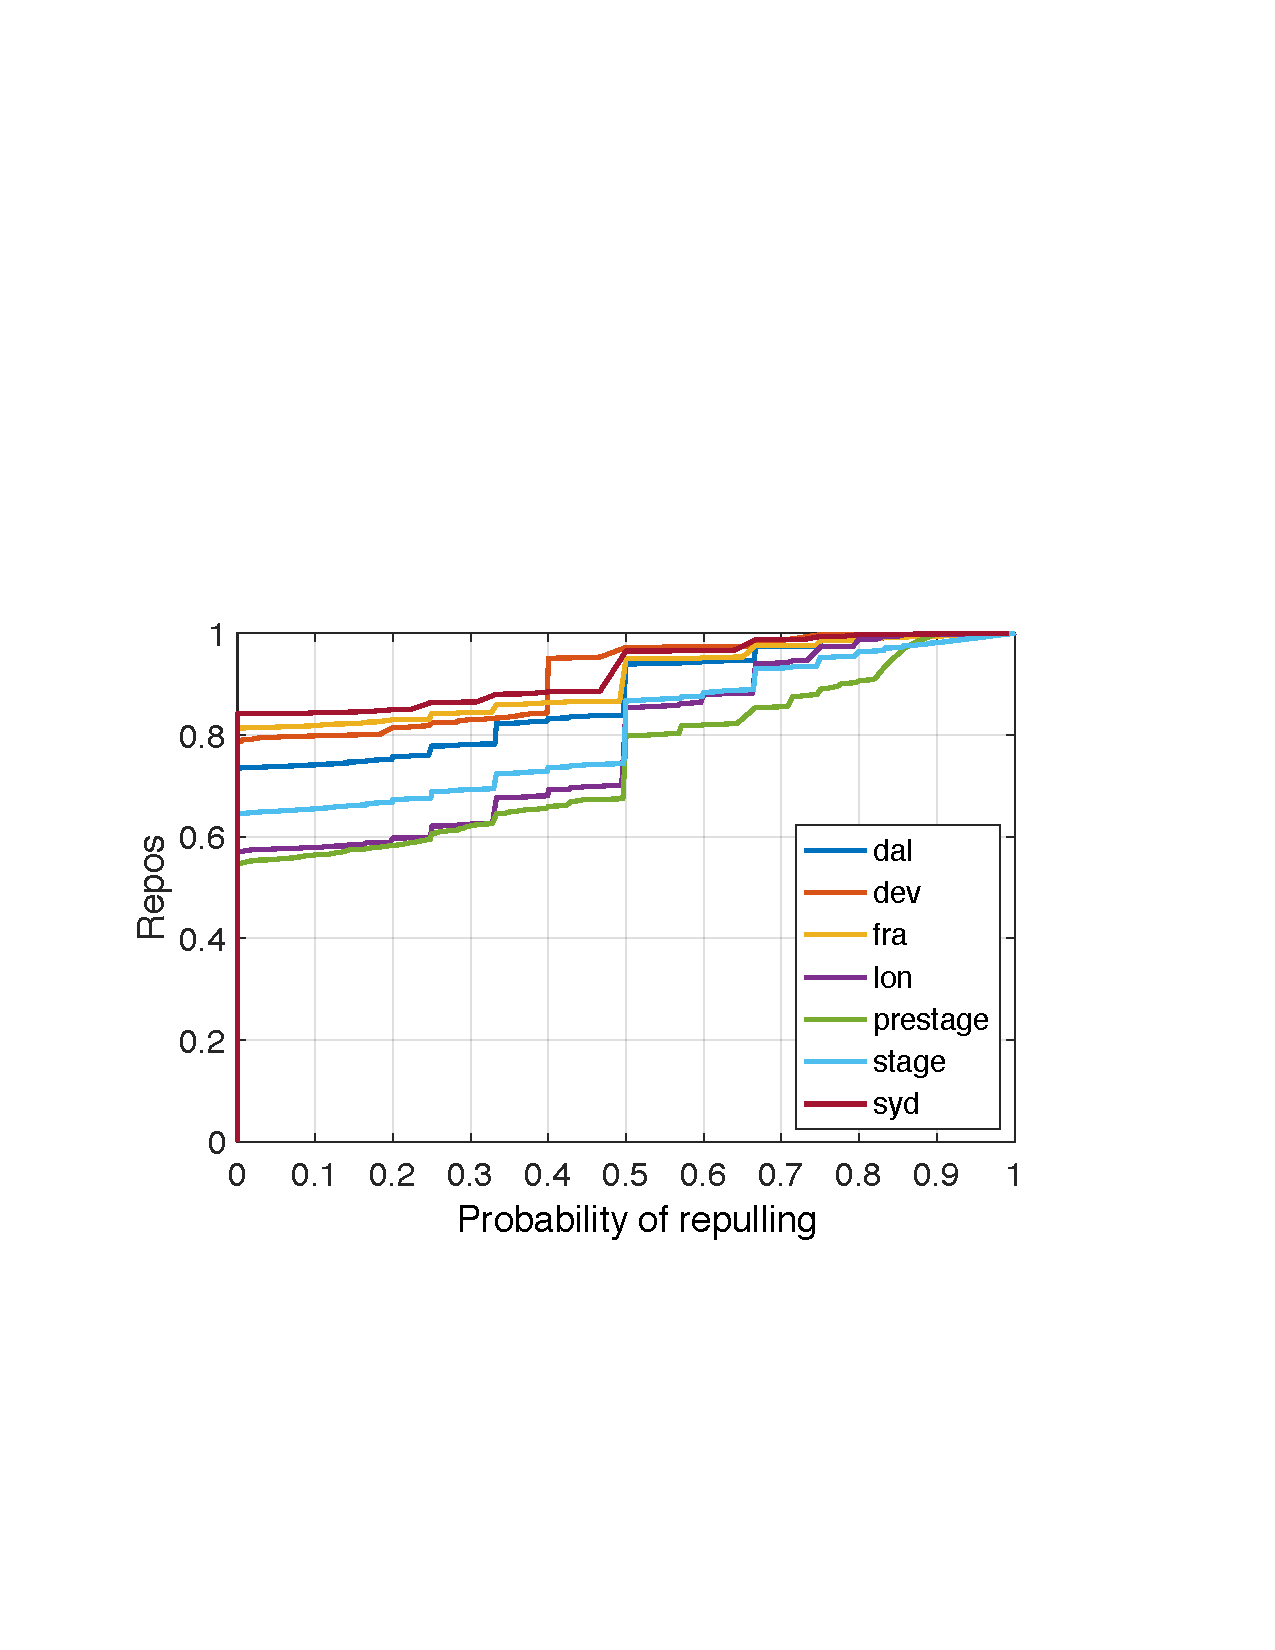
\includegraphics[width=0.2\linewidth]{graphs/cdf-repo-repull-ratio-by-same-client.pdf}
%%		\label{fig:repo-repull-cdf}
%%	}
%	\subfigure[Client repulling probability]{
%	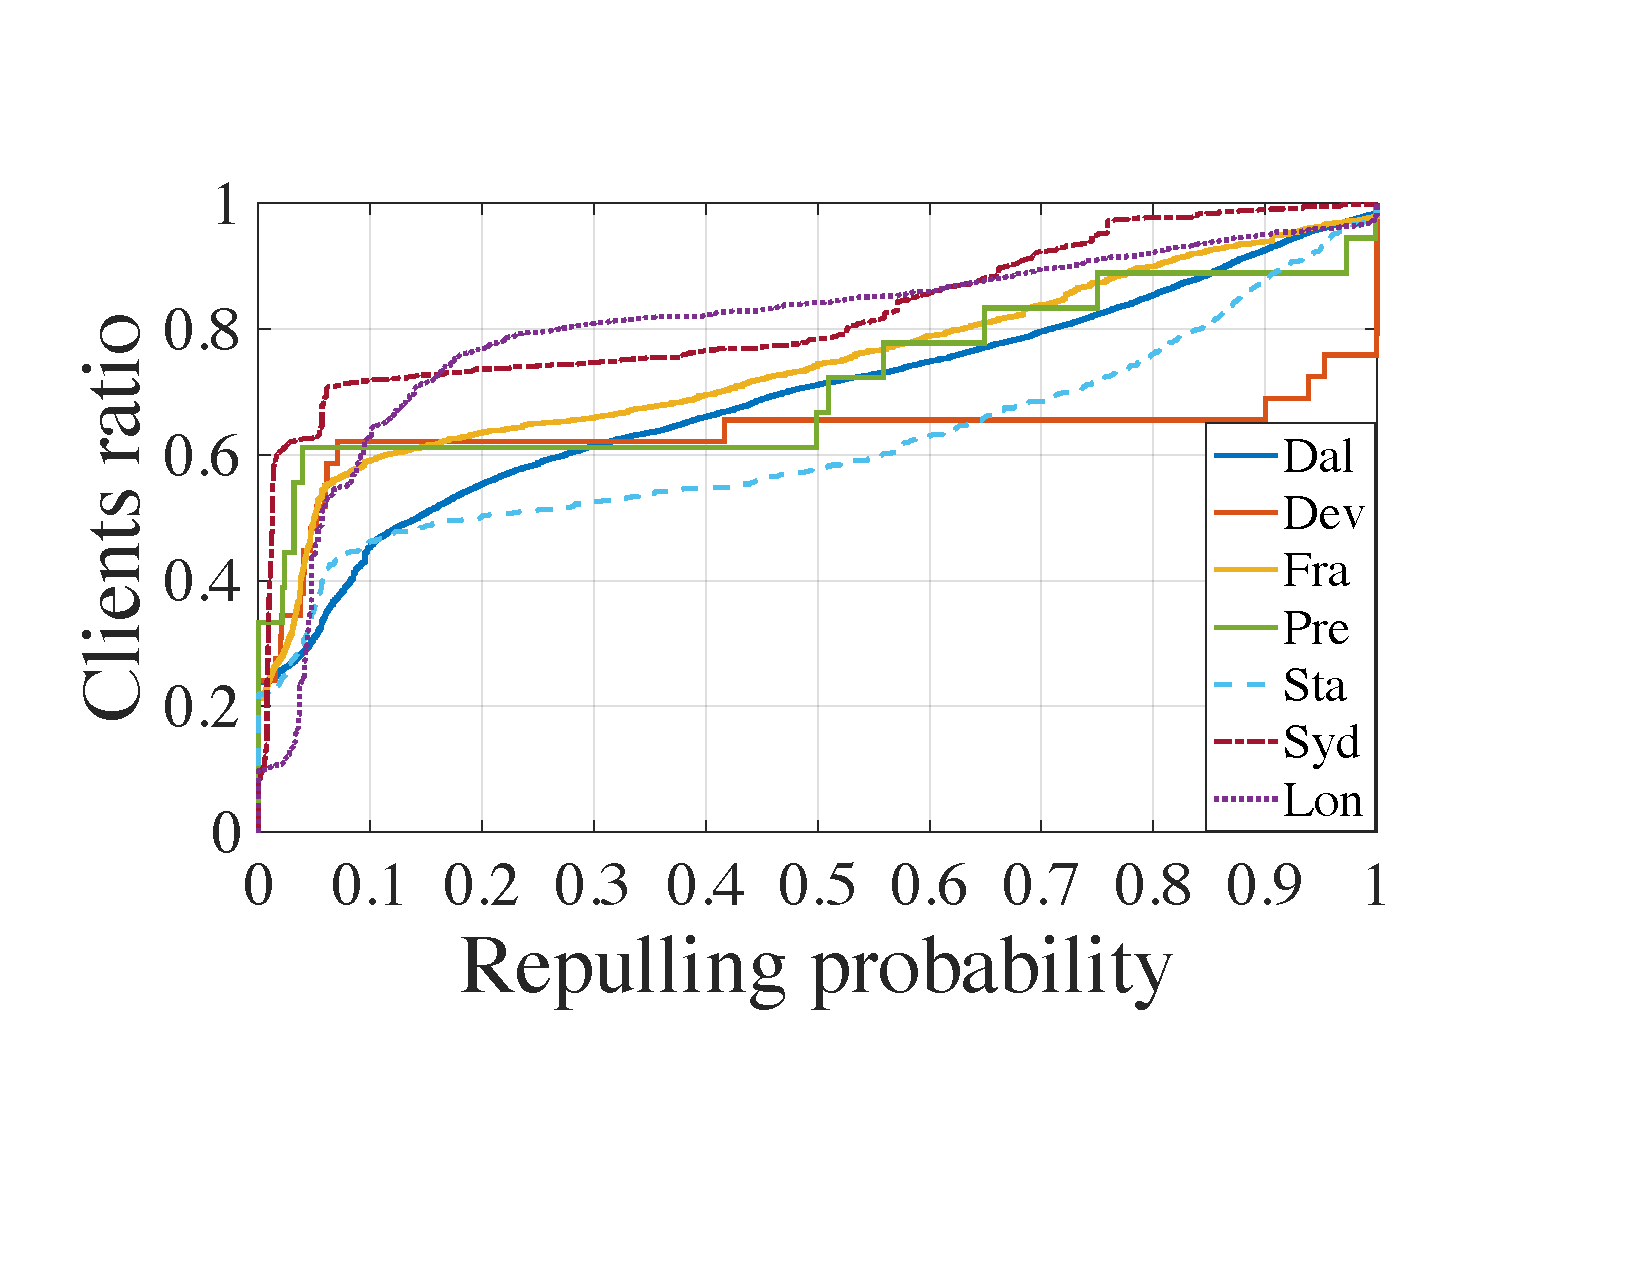
\includegraphics[width=0.2\textwidth]{graphs/cdf-client-repull-layer-request-ratio.pdf}
%   \label{fig:client-repull-cdf}
%}
%	\caption{CDF of \texttt{GET} layer request count and client repulling probability.}
%	\label{fig-repull}
%\end{figure}
%






\begin{figure*}[t]
        \centering
        \begin{minipage}{0.3\textwidth}
                \centering
                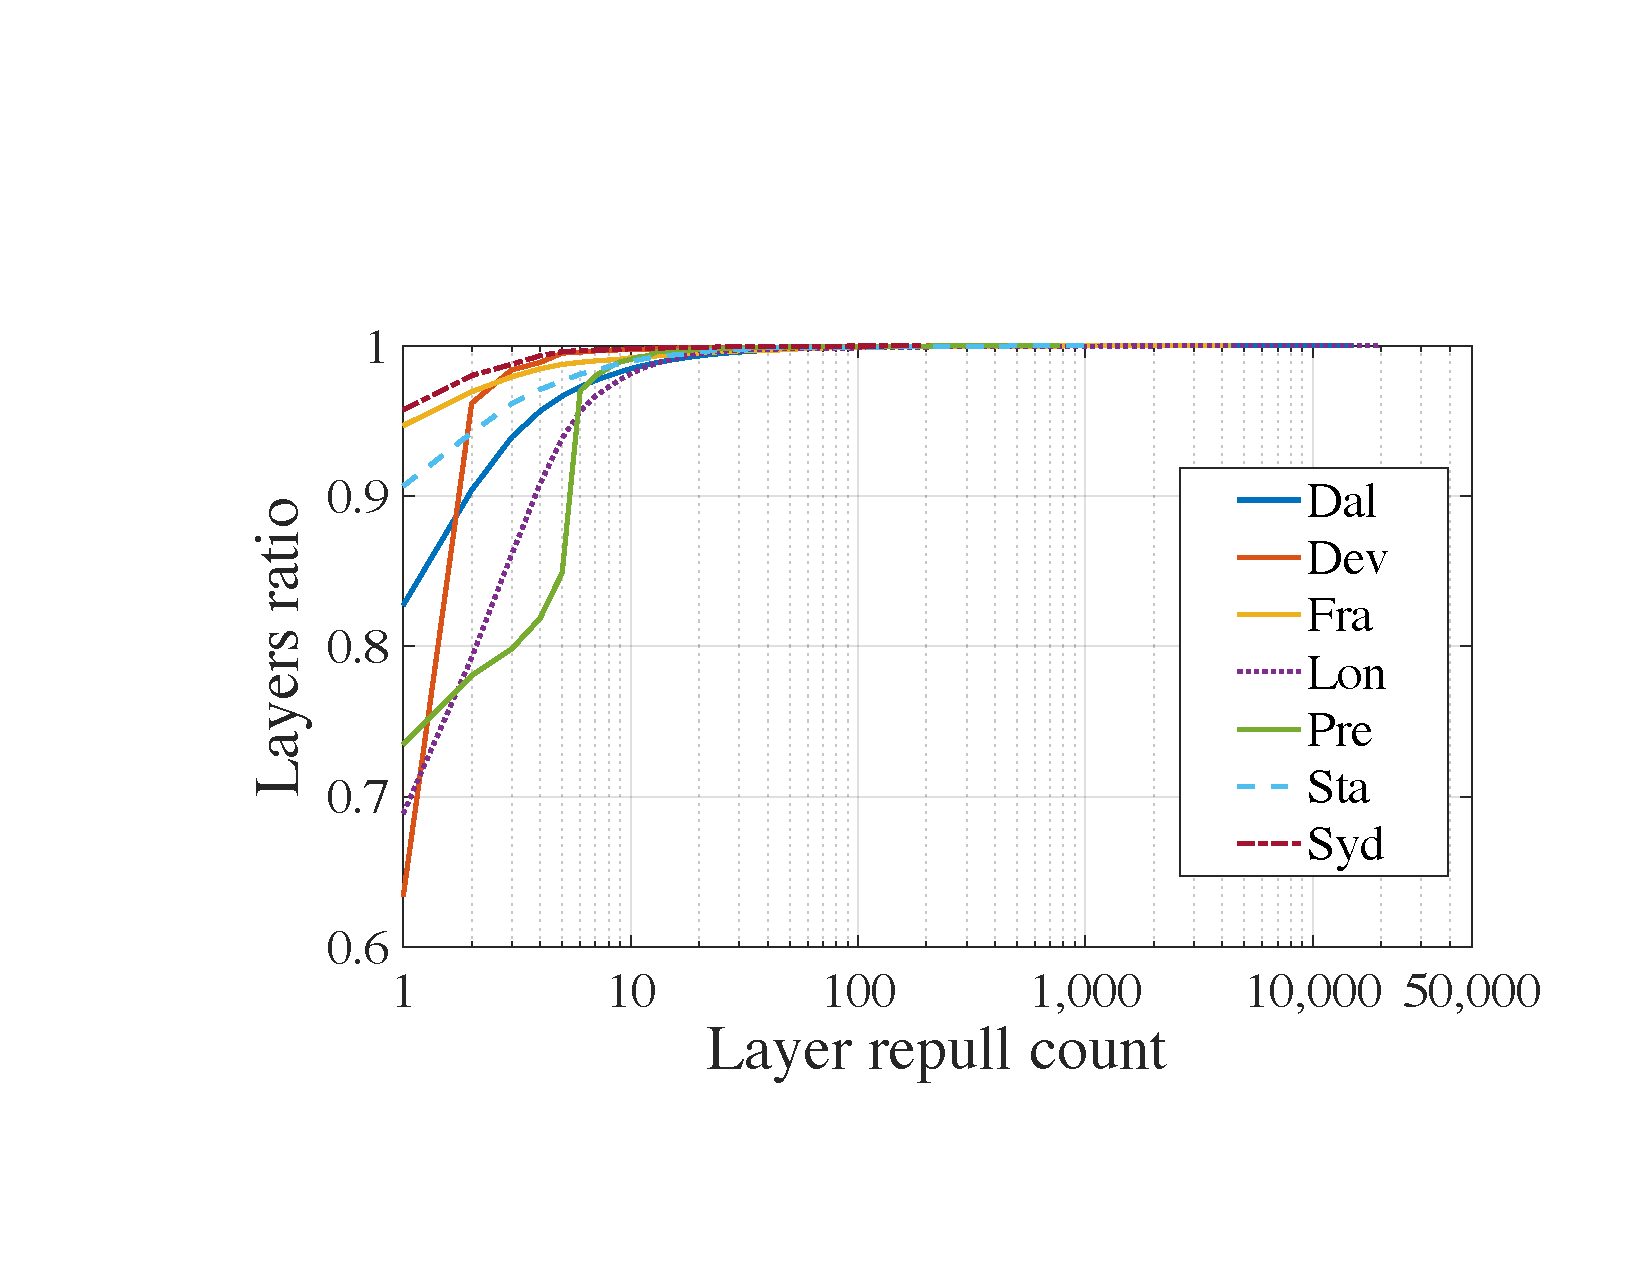
\includegraphics[width=0.9\textwidth]{{graphs/cdf-layer-repull-ratio-by-same-client.pdf}
                \caption{CDF of \texttt{GET} layer request count}
                \label{fig:layer-repull-cdf}
        \end{minipage}%
        \begin{minipage}{0.3\textwidth}
                \centering
                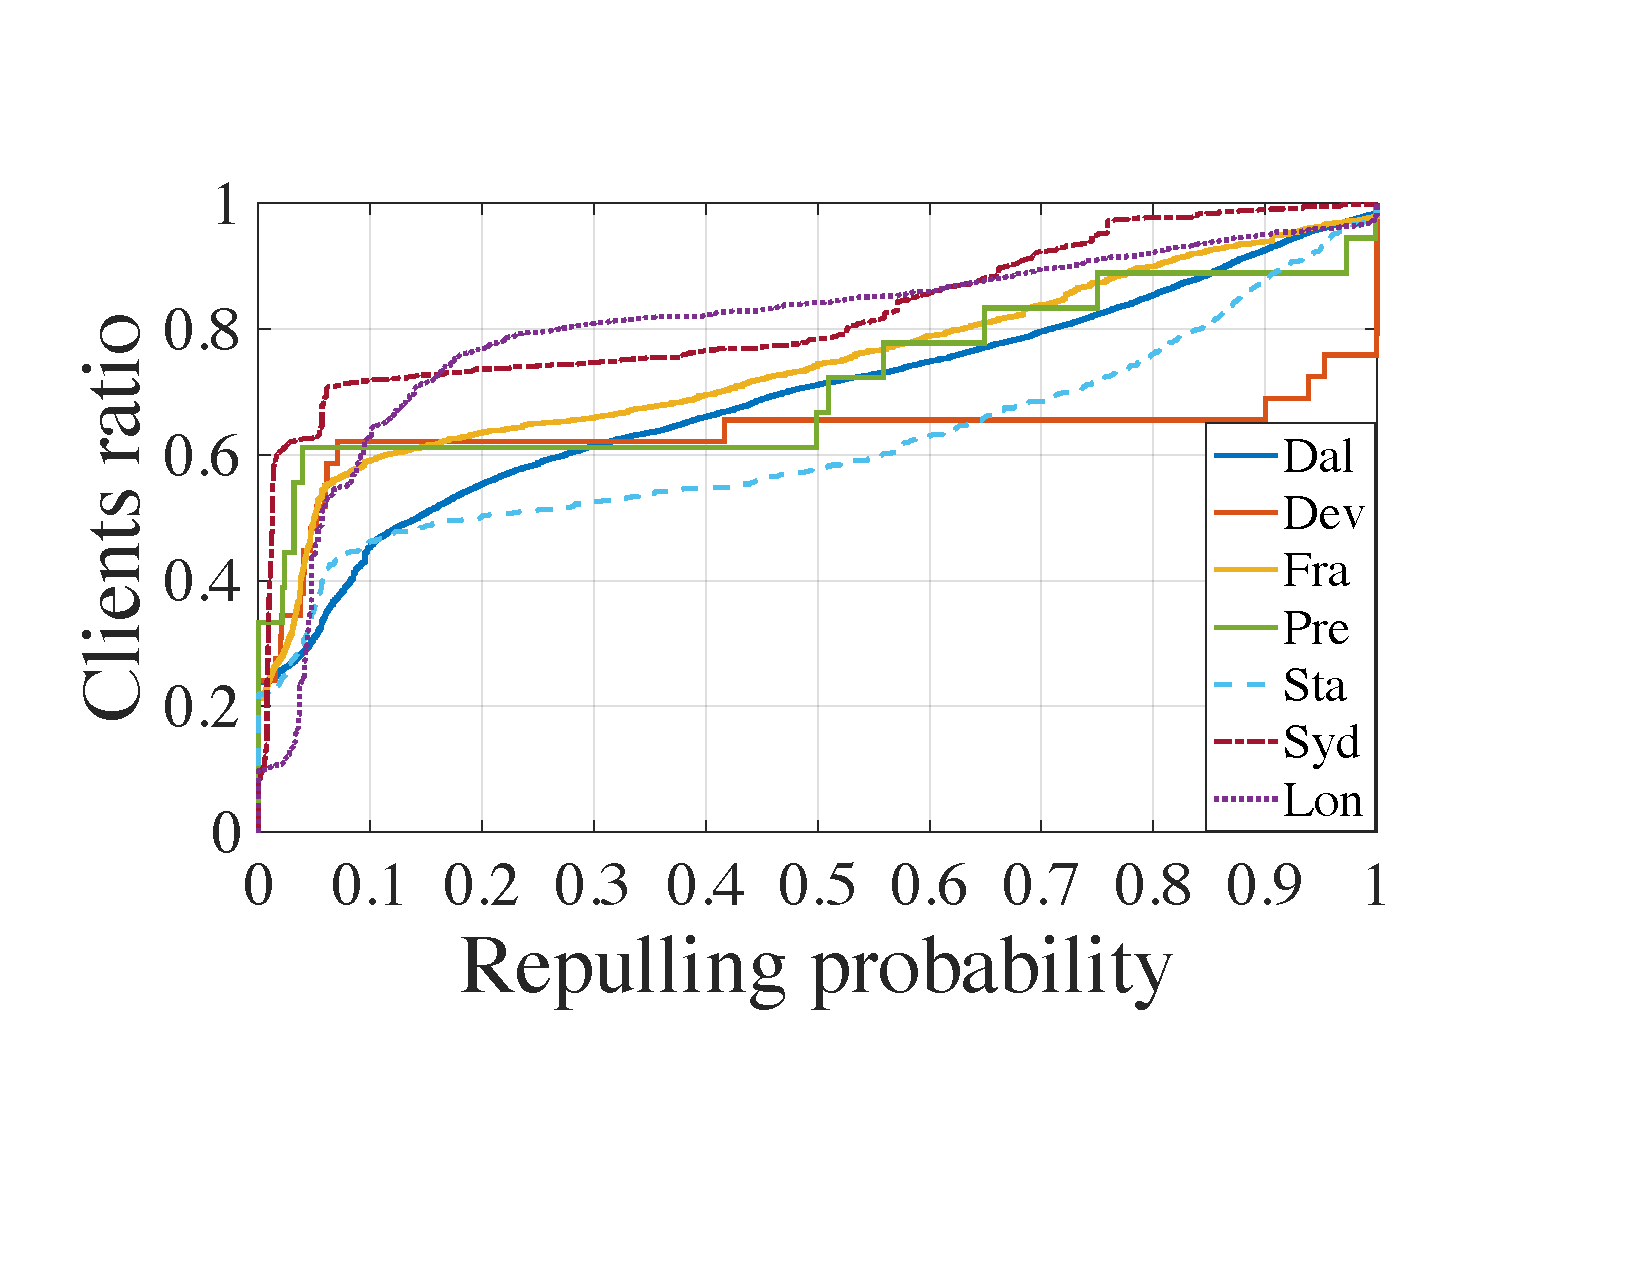
\includegraphics[width=0.9\textwidth]{graphs/cdf-client-repull-layer-request-ratio.pdf}
                \caption{CDF of Client repulling probability}% of LRU cache and preconstruct cache.}
                \label{fig:client-repull-cdf}
        \end{minipage}%
        \begin{minipage}{0.3\textwidth}
        \centering
        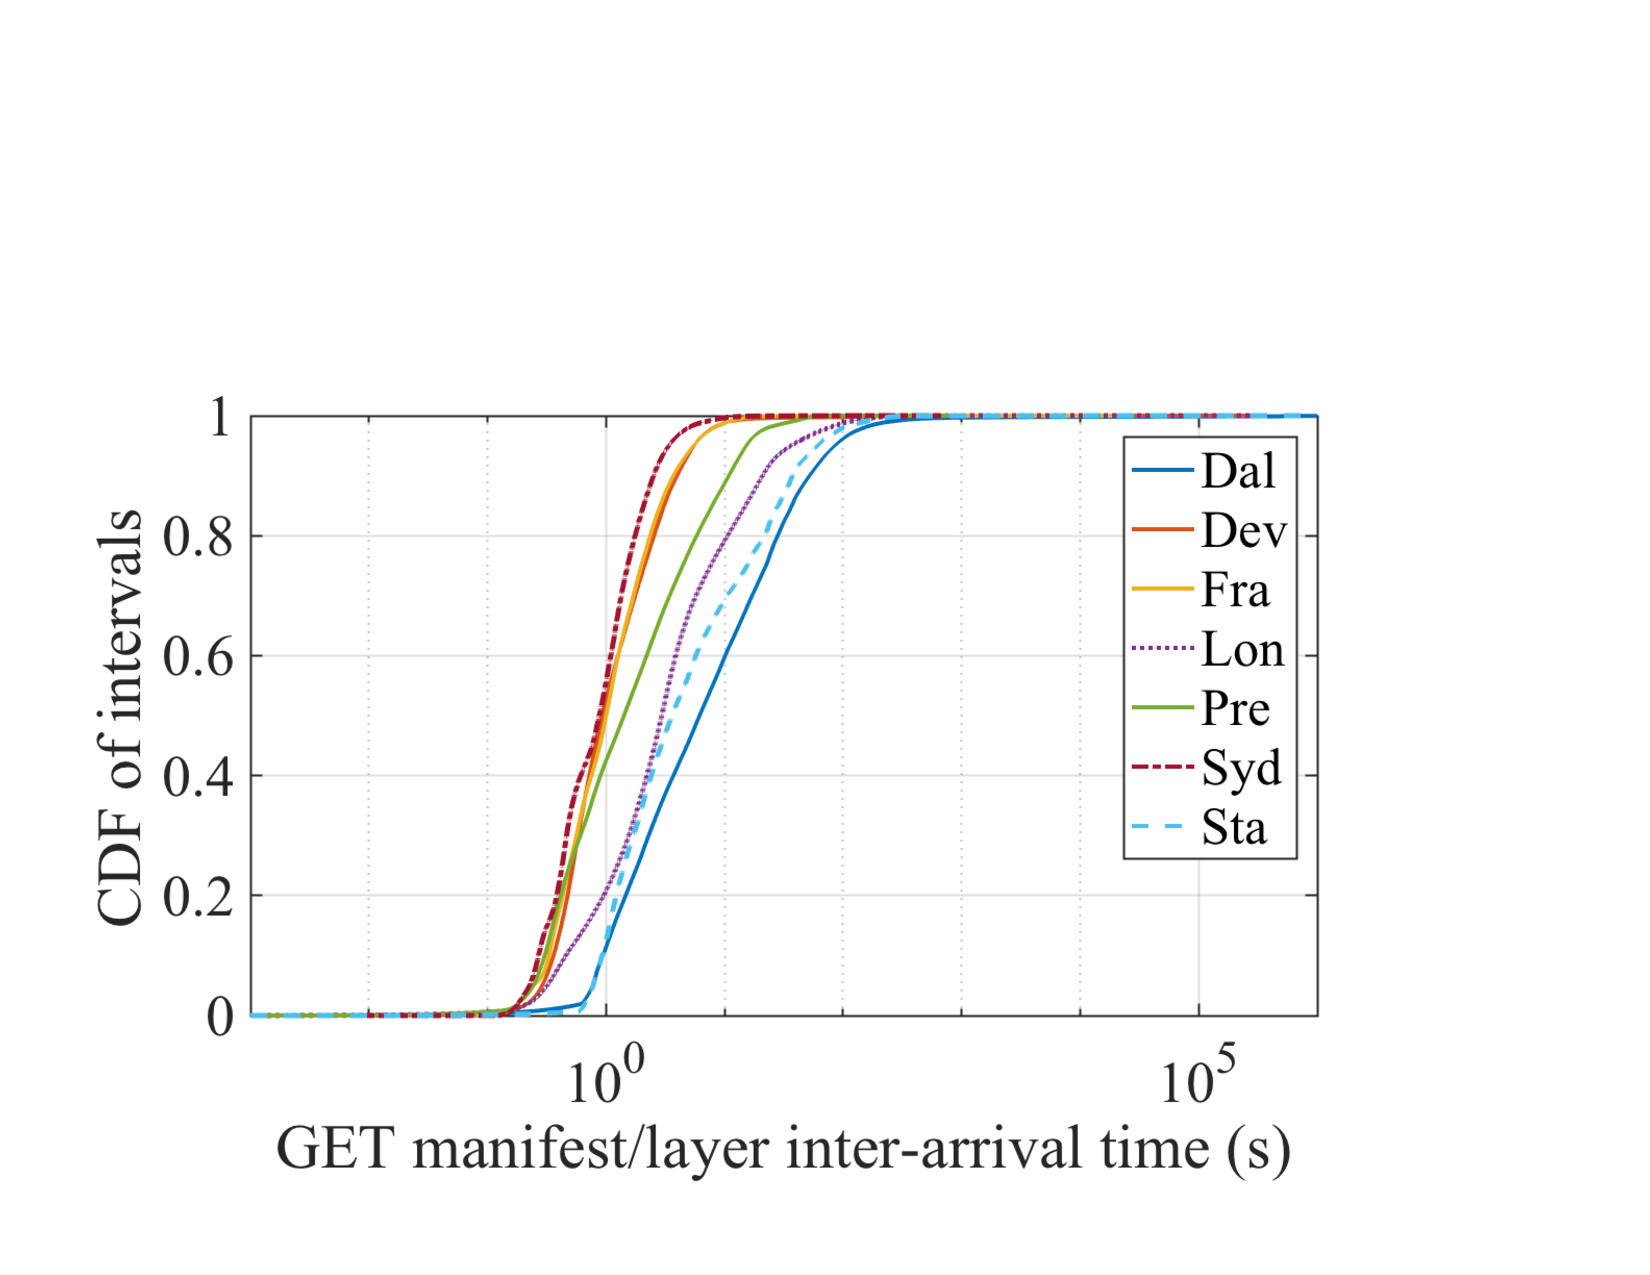
\includegraphics[width=0.9\textwidth]{graphs/GML-intervals.pdf}
        \caption{Intervals between \texttt{GET} manifest request and \texttt{GET} layer request}
        \label{fig:intervals}
   \end{minipage}
\end{figure*}





%\begin{figure}[!t]
%	\centering
%	\subfigure[CDF of compression ratio]{\label{fig_cdf_compression_ratio}
%		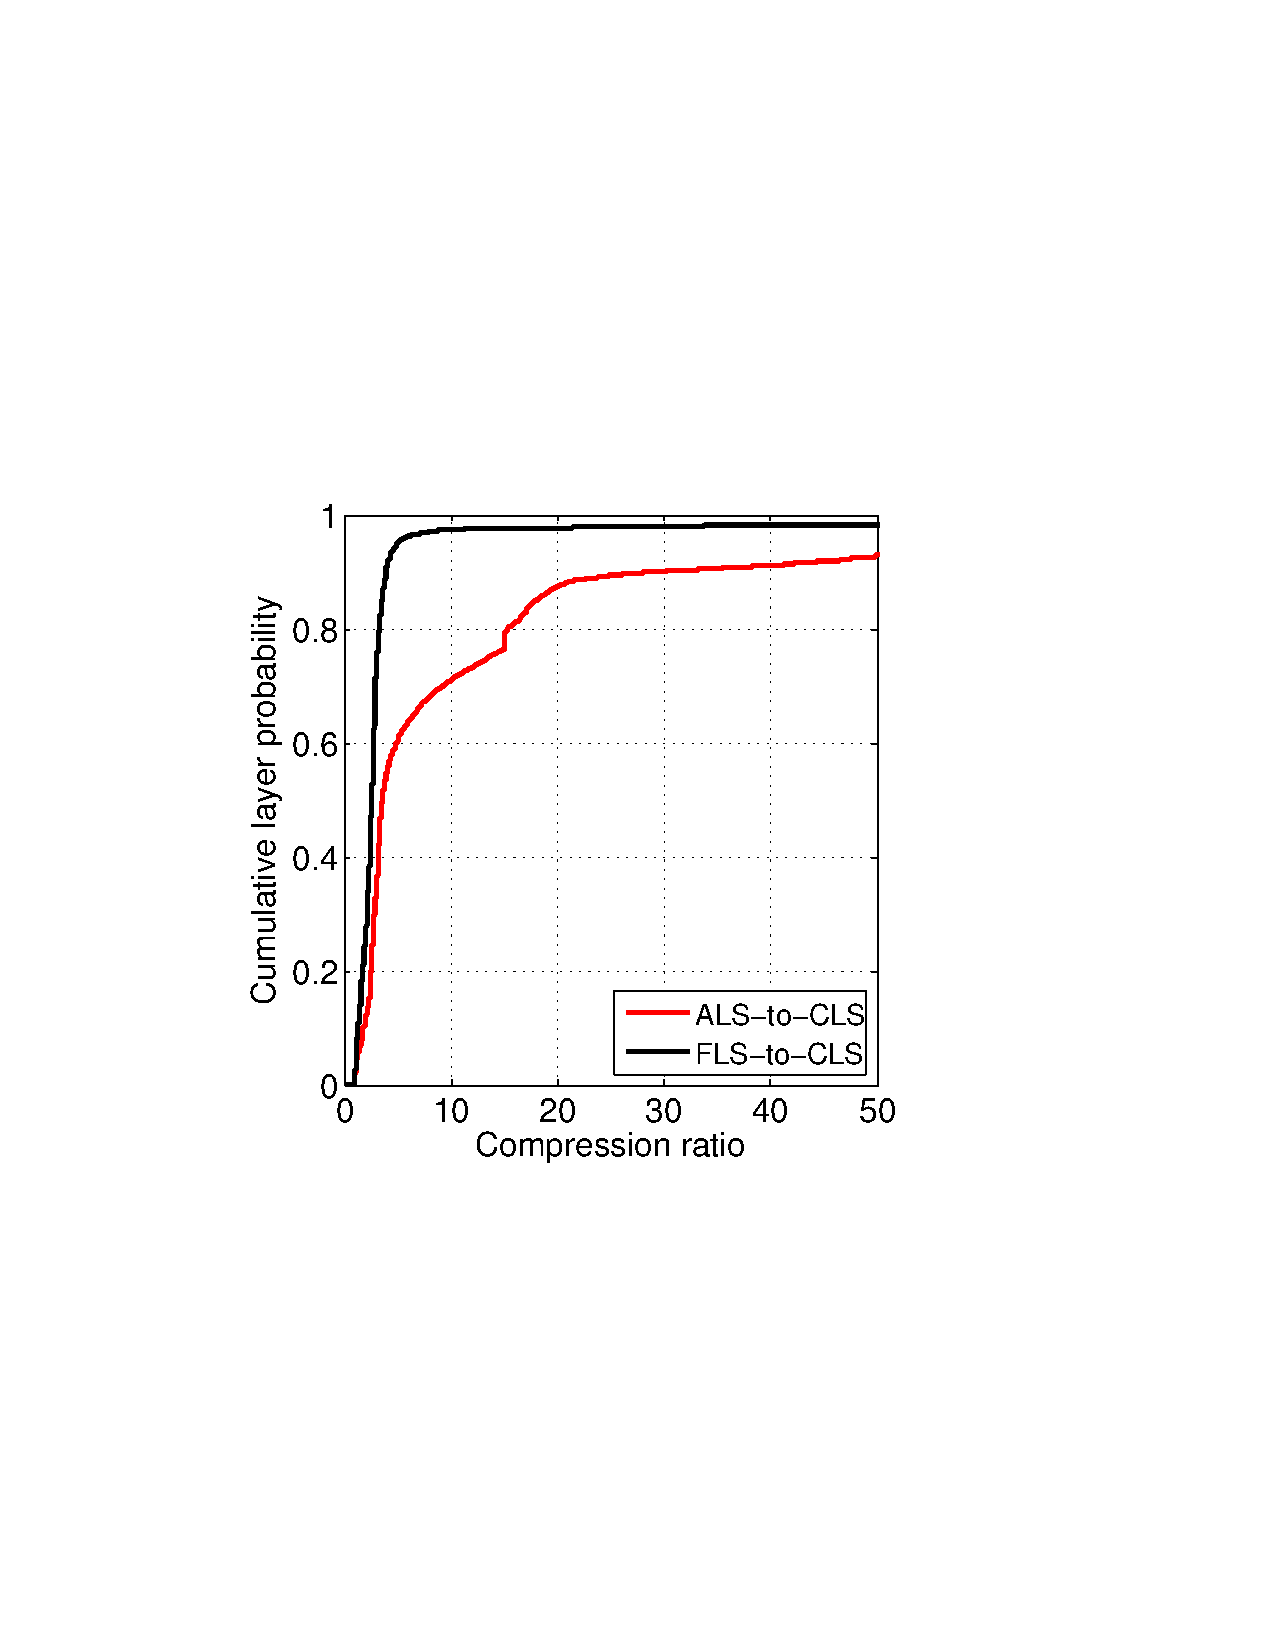
\includegraphics[width=0.23\textwidth]{graphs/cdf_compression_ratio.pdf}
%	}
%	\subfigure[Histogram of comp. ratios]{\label{fig_his_compression_ratio}
%		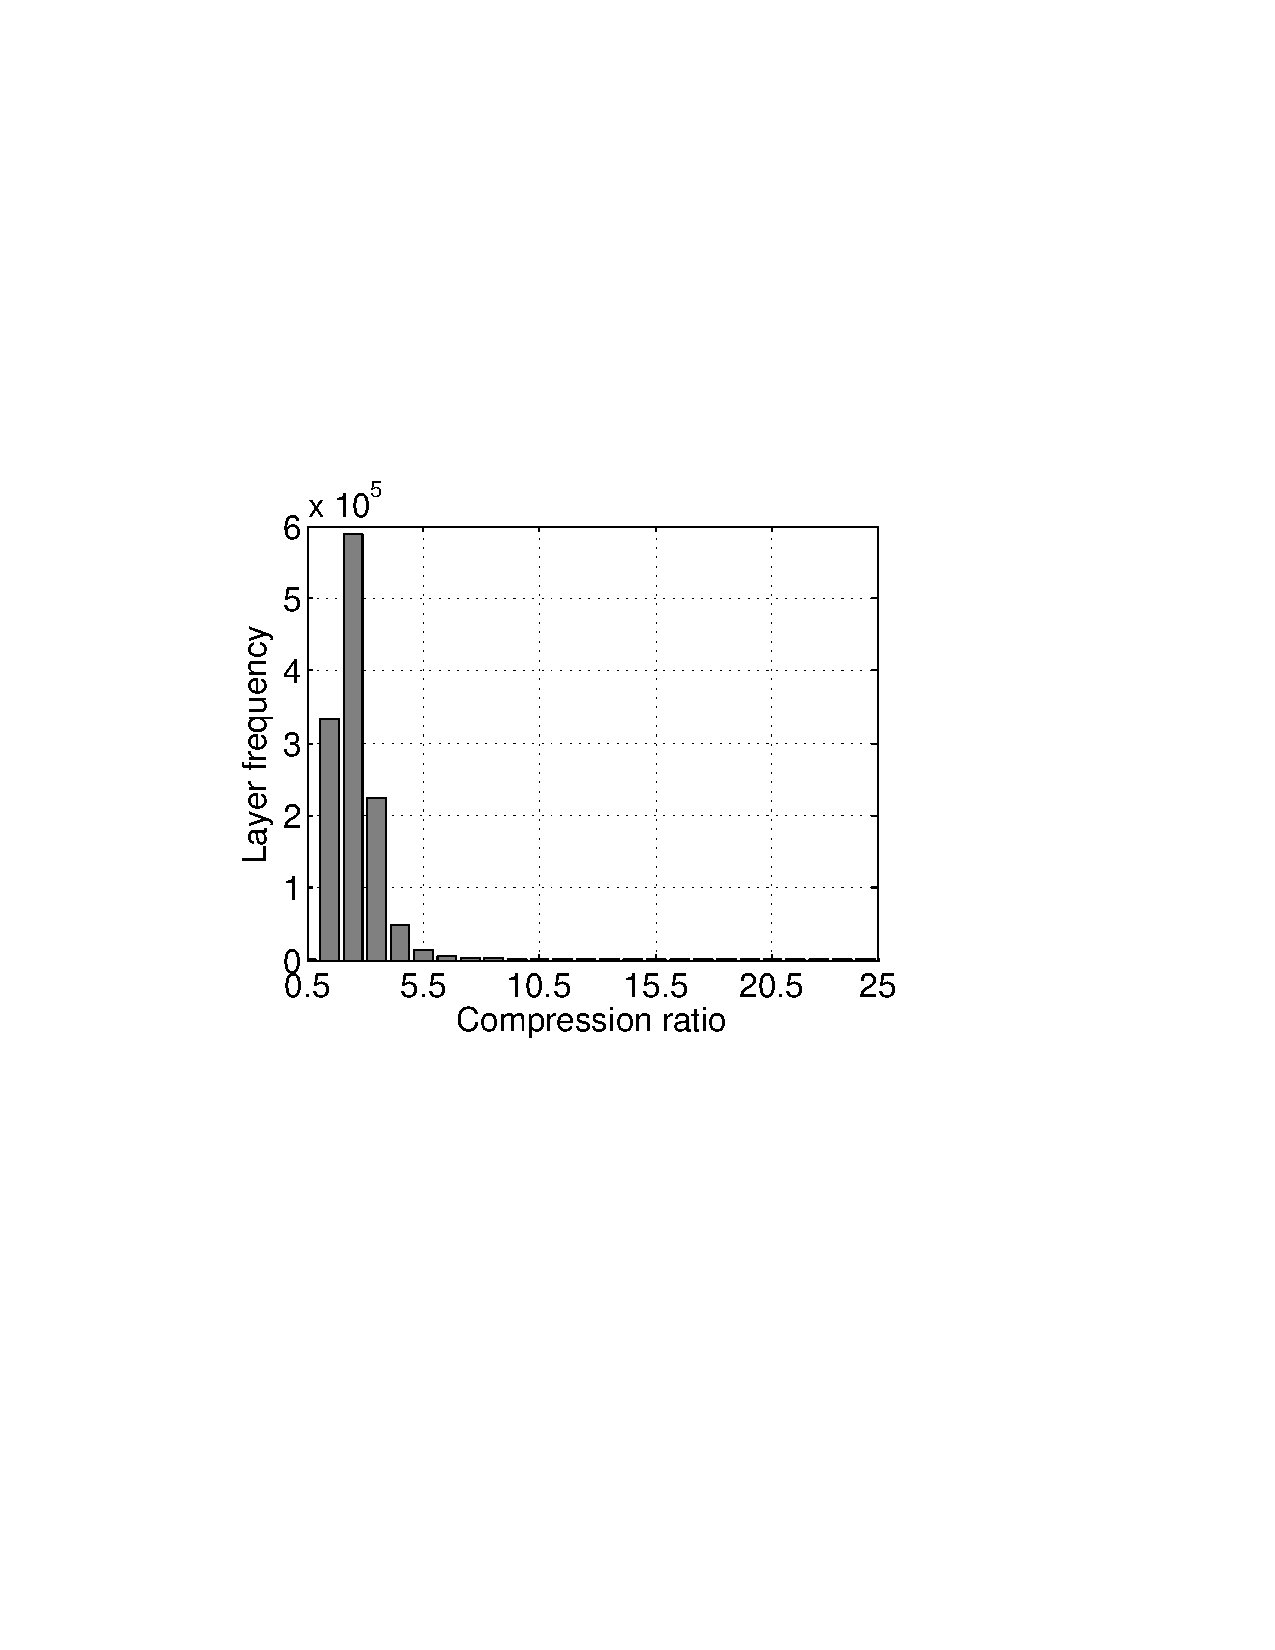
\includegraphics[width=0.223\textwidth]{graphs/his_compression_ratio.pdf}
%	}
%	\caption{Layer compression ratio distribution
%		%\vcomment{Different colors are used in figure (a) and (b) FLS/CLS\nancomment{will address later}}
%	}
%	\label{fig-compression-ratio}
%\end{figure}


%\begin{figure}[t]
%	\centering
%	\begin{minipage}{0.26\textwidth}
%		\centering
%		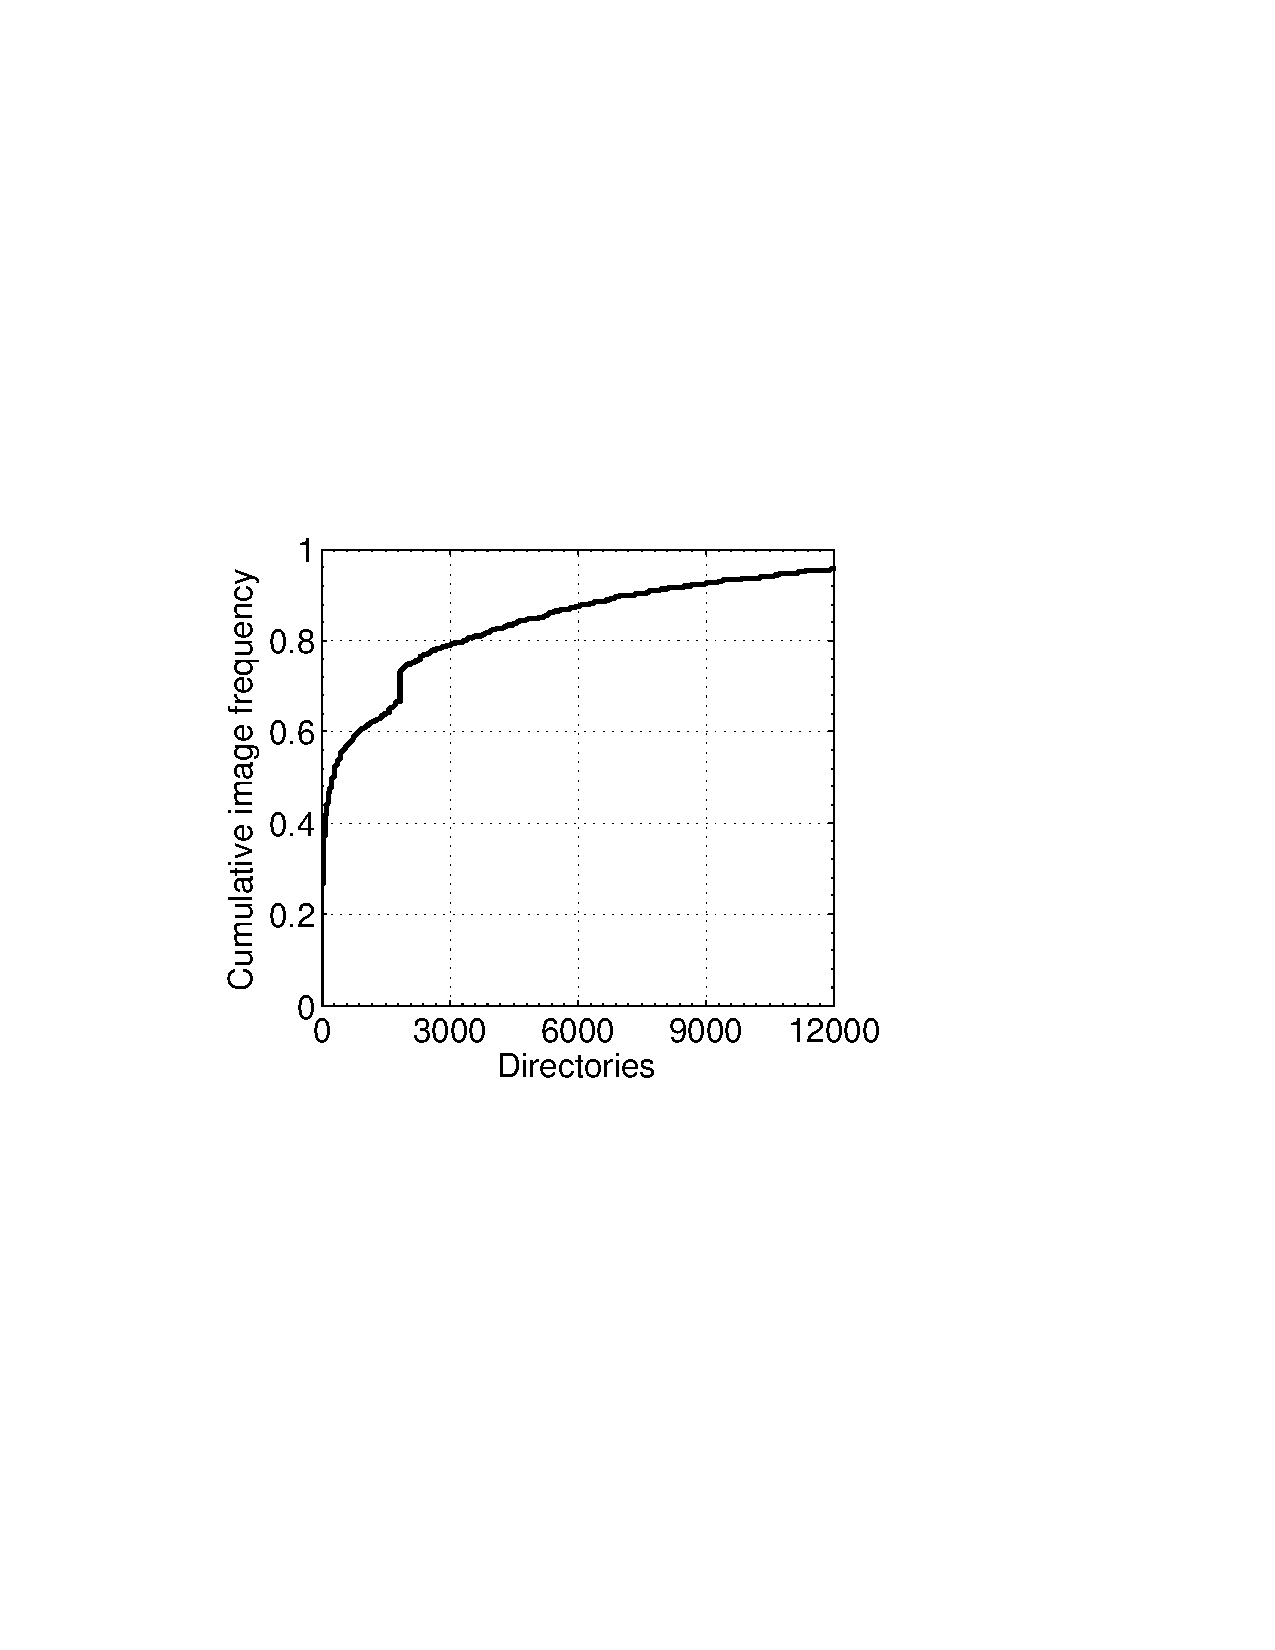
\includegraphics[width=1\textwidth]{graphs/dir.pdf}
%		\caption{CDF of images by\newline directories}
%		\label{fig-dir}
%	\end{minipage}%
%	\begin{minipage}{0.24\textwidth}
%		\centering
%		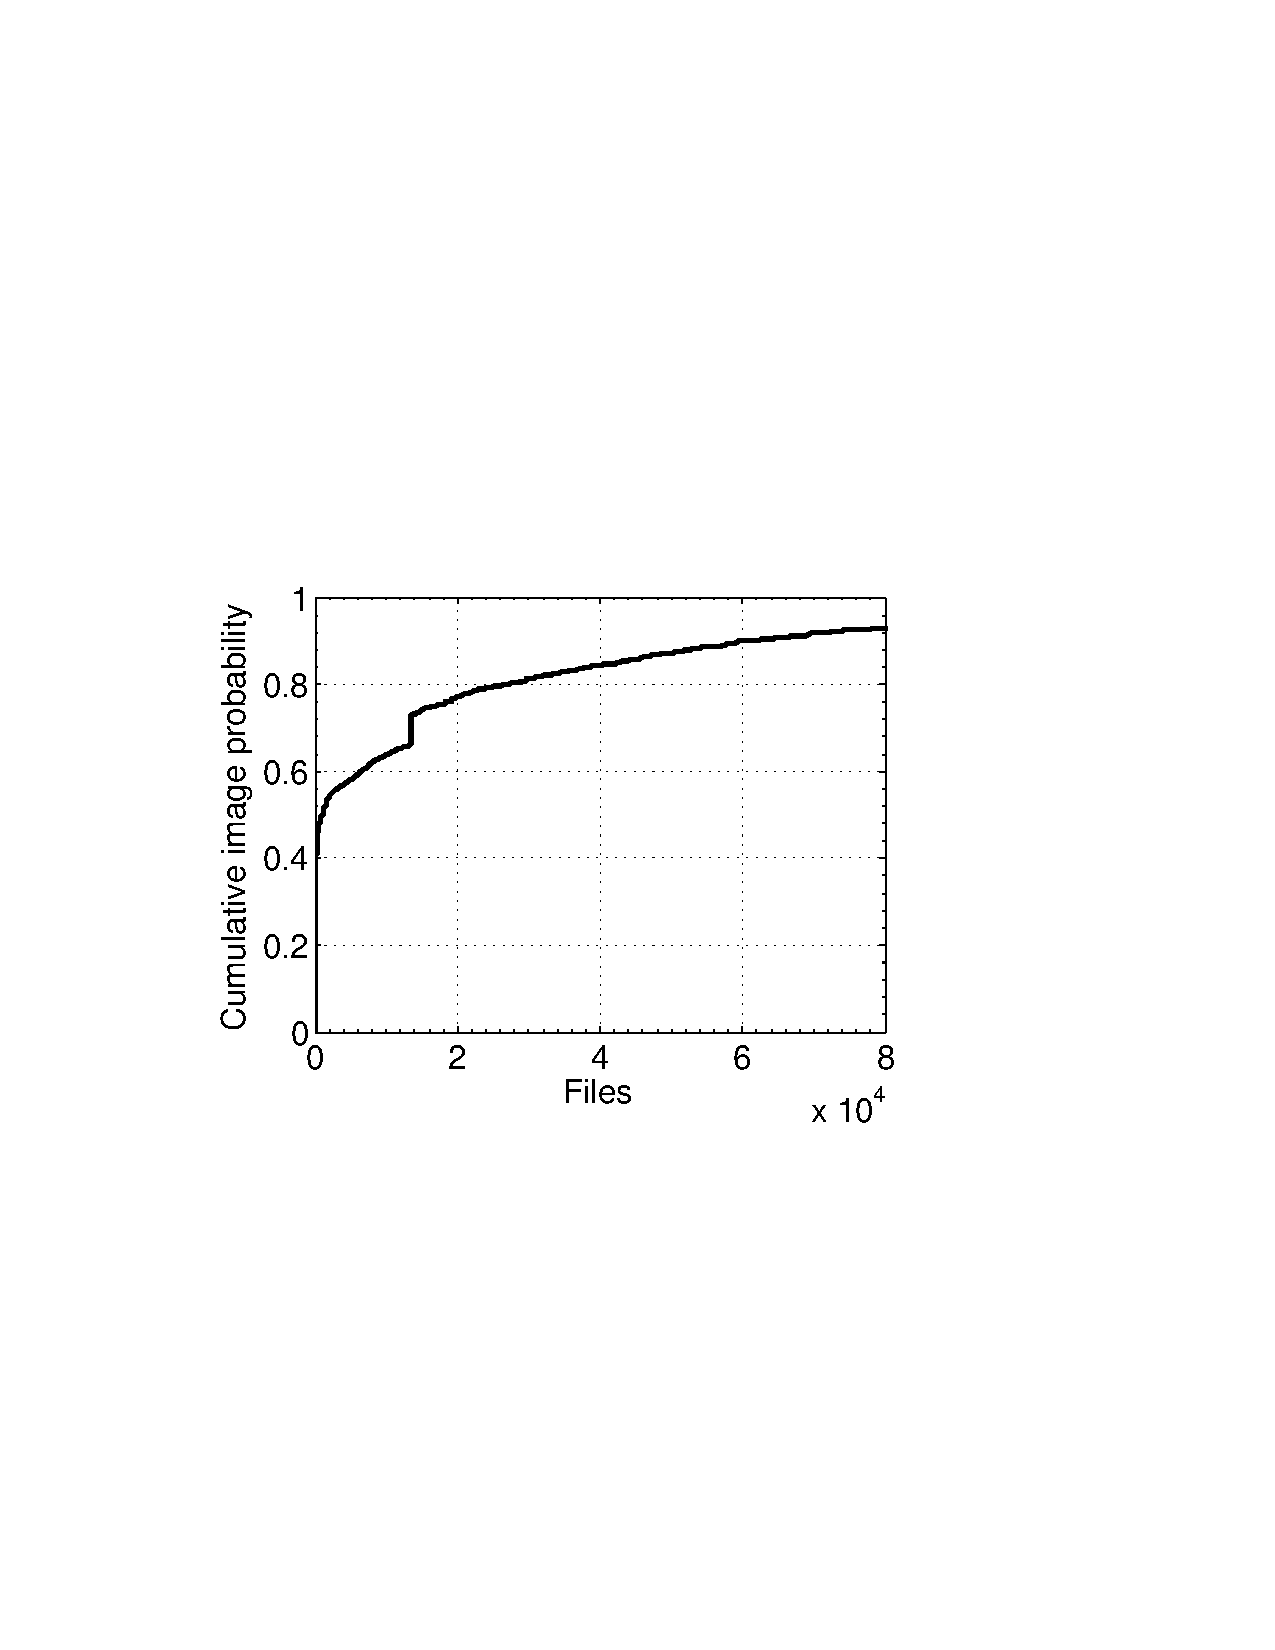
\includegraphics[width=1\textwidth]{graphs/file.pdf}
%		\caption{CDF of images by files}
%		\label{fig-file}
%	\end{minipage}
%\end{figure}

%\begin{figure}[htbp] 
%	\begin{minipage}{0.5\linewidth} 
%		\centering 
%		\includegraphics{circle} 
%		\caption{A Circle} 
%		\label{fig:circle} 
%	\end{minipage}% 
%	\begin{minipage}{0.5\linewidth} 
%		\centering 
%		\includegraphics{rectangle} 
%		\caption{A Rectangle} 
%		\label{fig:rectangle} 
%	\end{minipage} 
%\end{figure}
